\chapter{Analysis and Design of the Automated Log Analysis Pipeline}

This chapter presents the analysis and design of the proposed automated log analysis system. It describes the design specifications, the pre-analysis work carried out before the implementation, the four-stage design methodology (data collection, log processing, analysis engine, output \& delivery), and the design equations used for performance metric computation. The performance parameters extracted from each log and the reference test suite are also documented in detail.

\section{Contents of this Chapter}
This chapter contains the following sections and subsections in detail.
\begin{enumerate}
\item Specifications for the Design
\item Pre-analysis work for the design or Models used
\item Design methodology in detail
\item Design Equations
\item Experimental techniques (test suite and configurations under test)
\end{enumerate}

\subsection{Specifications for the Design}
The system is designed to satisfy the following specifications:
\begin{itemize}
\item Process more than one hundred log files per regression run without manual intervention.
\item Produce a per-regression three-sheet Excel workbook (raw metrics, derived metrics and summary) for every option under test.
\item Produce a final multi-option comparison workbook that places the Cascade baseline alongside Nova-Alpha through Nova-Epsilon.
\item Compute percentage difference of every metric against the baseline and flag degraded tests automatically.
\item Provide an LLM-generated summary and a root-cause hint for every degraded test.
\item Limit total wall-clock time to approximately two minutes per regression on the standard development server.
\end{itemize}

\subsection{Pre-analysis Work and Models Used}
Before the design, a study of the existing manual workflow was carried out. The engineer would (i) navigate to the log directory of the option under test, (ii) grep for cycles, IPS, bandwidth and stall counters, (iii) copy the values into a spreadsheet, (iv) compute percentage differences manually and (v) write a short summary. This manual flow was profiled and used as the baseline against which the automated pipeline is benchmarked. On a typical run with twelve graphs across six options, this manual workflow took between one and a half and three hours per regression, with most of the time spent on grepping, transcription and spreadsheet formatting rather than on technical analysis.

The pre-analysis also identified two recurring sources of error in the manual flow. First, transcription errors when copying multi-digit counter values from terminal output to spreadsheet cells, which sometimes propagated to the final degradation report. Second, inconsistency across engineers in how counters were named and aggregated, so that two regressions reported by two different engineers could not always be compared cell-to-cell. The proposed pipeline eliminates both classes of error by using deterministic regular expressions and a single canonical column schema.

The models used in the pipeline are: the Drain template parser from LogPAI, K-means clustering and isolation-forest based anomaly detection from LogAI, and an LLM (GPT/Claude) accessed via API for text summarization. Regular expressions handle the deterministic counters whose format is known and stable. The Drain parser is configured with a similarity threshold and a tree depth that were tuned empirically on a representative subset of three hundred log lines drawn from the test suite. The LogAI clustering step groups parsed log templates by their numerical feature vectors so that anomalous events stand out without the need for hand-labelled training data.

\subsection{Design Methodology in Detail}
The design methodology consists of four stages that are executed in sequence per regression run.

\subsubsection{Stage 1 - Data Collection}
The data collection stage begins with the execution of software test cases on the emulation platform. The platform produces raw log files for each test, which are then collected and stored in a structured directory tree (one directory per option under test, containing one log file per graph). Once all logs are present, the stage signals \textit{Log Data Ready} for the next stage. Figure \ref{fig:datacoll} shows the flow of this stage, in which the test execution, log generation and log ingestion paths converge into a single \textit{Log Data Ready} node that gates the downstream stages.

\begin{figure}[htb]
\centering
	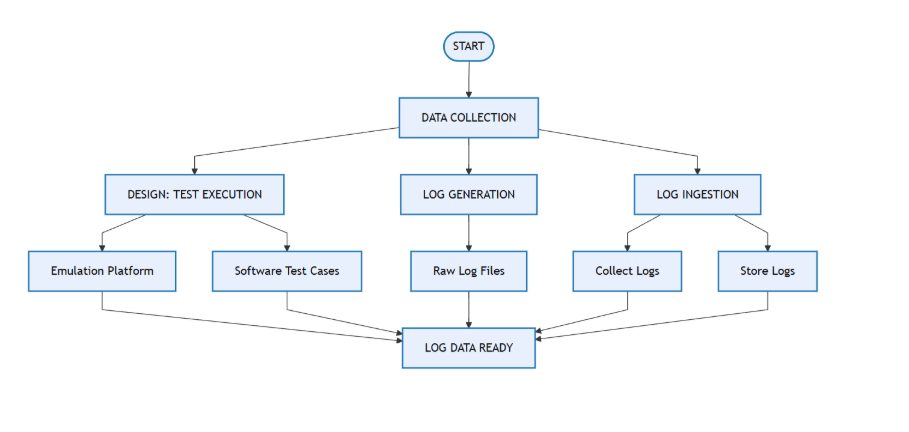
\includegraphics[width=0.9\textwidth]{Figures/fig1}
	\caption{Data collection stage of the proposed pipeline}
	\label{fig:datacoll}
\end{figure}

The directory layout used for storage mirrors the option-graph hierarchy: \texttt{<regression\_id>/<option>/<graph>.log}. This layout is chosen so that the downstream comparison engine can iterate over graphs and pivot across options without any extra metadata file. The ingestion module also writes a small manifest that records the timestamp of each log, the build identifier of the emulation image and the random seed used for the test, so that any regression can be reproduced bit-exactly later.

\subsubsection{Stage 2 - Log Processing}
The log processing stage takes the raw log files as input and produces structured logs and feature vectors. It consists of three parallel paths: a preprocessing path that normalizes and cleans the raw text, a parsing path that uses LogPAI's Drain algorithm to extract templates, and a feature extraction path that builds numeric feature vectors for downstream ML. The flow is shown in Figure \ref{fig:logproc}.

\begin{figure}[htb]
\centering
	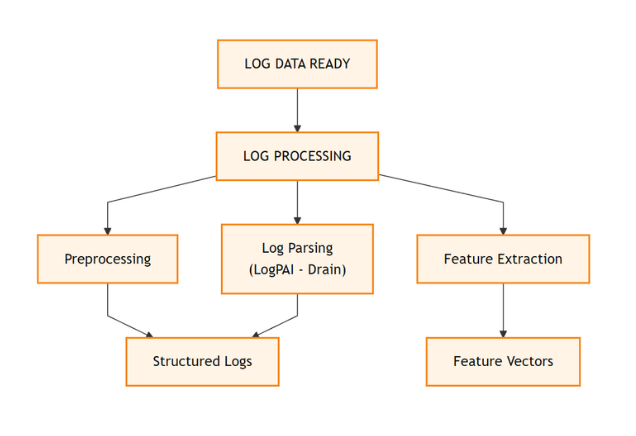
\includegraphics[width=0.7\textwidth]{Figures/fig2}
	\caption{Log processing stage of the proposed pipeline}
	\label{fig:logproc}
\end{figure}

The preprocessing path strips timestamps, ANSI colour codes and platform banner lines so that the parser sees a clean stream. The Drain parser then performs token-based template extraction by walking a fixed-depth parse tree, where each leaf corresponds to a unique template. New log lines that do not match any existing template at the configured similarity threshold are added as new leaves, allowing the parser to grow its template set incrementally. Once parsed, each log line is replaced by a (template ID, parameter list) pair that downstream stages consume. The feature extraction path operates in parallel on the raw counters and produces fixed-length numeric vectors that summarize the activity of each test, which feed both the clustering and the metric-extraction sub-modules of the analysis engine.

\subsubsection{Stage 3 - Analysis Engine}
The analysis engine is the heart of the pipeline. It consumes the structured logs and feature vectors and is composed of three sub-modules executing in parallel: a Log Analysis sub-module (LogAI) that performs clustering and anomaly detection; a Metric Extraction sub-module that pulls bandwidth, clock cycles, IPS, pass/fail status and a regression comparison block (baseline vs.\ options) that produces a degradation summary in terms of percentage difference and counts; and an LLM Analysis sub-module that performs summary generation and root-cause analysis. Figure \ref{fig:analysisengine} captures the internal structure of the engine.

\begin{figure}[htb]
\centering
	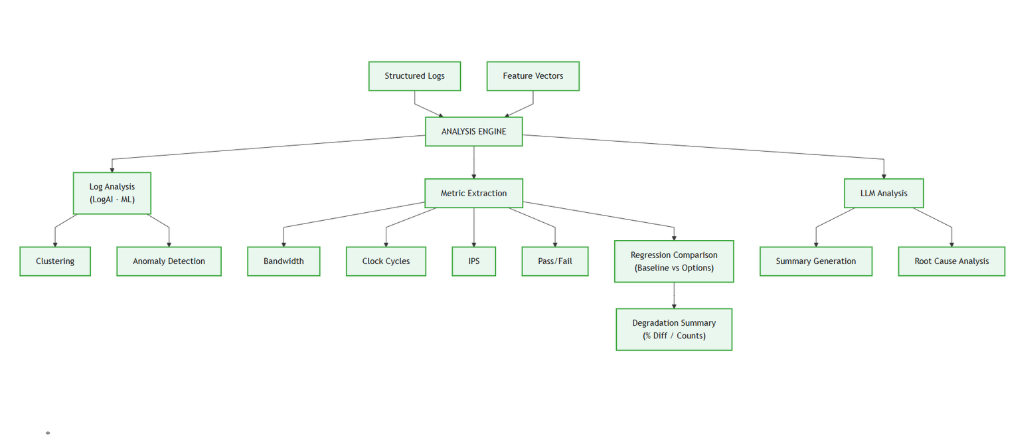
\includegraphics[width=\textwidth]{Figures/fig3}
	\caption{Analysis engine of the proposed pipeline}
	\label{fig:analysisengine}
\end{figure}

The Log Analysis sub-module uses K-means to cluster log templates and isolation-forest to flag anomalous events. The Metric Extraction sub-module is the most heavily used path in production: it applies the curated regular expressions described in Section \ref{sec:params} to extract bandwidth, cycles, IPS and the full set of stall and parallelism counters. The Regression Comparison block then computes percentage differences against the Cascade baseline using Equation \ref{eqn:pctdiff} and emits a Degradation Summary with per-option counts. Finally, the LLM Analysis sub-module assembles a compact prompt for every degraded test and asks the model to produce a one-line summary and a directional root-cause hint, which become part of the per-regression workbook.

\subsubsection{Stage 4 - Output and Delivery}
The output \& delivery stage takes the clustering / anomaly results, the degradation summary and the LLM summary / root-cause analysis, and produces two artifacts: a Report Generation path that writes CSV and XLSX reports and a dashboard, and a Notification System path that produces email alerts and status updates. Once the artifacts are produced, the regression flow ends. Figure \ref{fig:output} shows the merge of the three analysis outputs into the two downstream paths.

\begin{figure}[htb]
\centering
	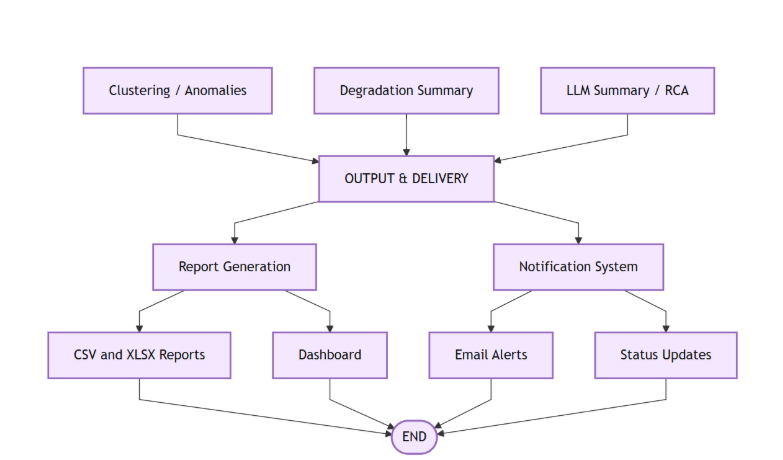
\includegraphics[width=0.85\textwidth]{Figures/fig4}
	\caption{Output and delivery stage of the proposed pipeline}
	\label{fig:output}
\end{figure}

The Excel workbook produced for each option contains three sheets: a \textit{raw} sheet with every counter extracted from every log, a \textit{derived} sheet with computed quantities (percentage differences, ratios) and a \textit{summary} sheet that lists only the metrics that crossed the degradation threshold. A separate multi-option comparison workbook places the Cascade baseline alongside Nova-Alpha through Nova-Epsilon for cross-configuration analysis. The notification system posts the workbook link to a project channel and sends a short email digest to the validation lead that highlights the count of degraded tests and the worst-degraded graph for each option.

\subsection{Design Equations}
The percentage difference of a metric \textit{m} on option \textit{o} against the baseline (Cascade) is computed as in Eqn.\ \ref{eqn:pctdiff}:
\begin{equation}
\label{eqn:pctdiff}
\Delta_{m,o} = \frac{m_o - m_{\text{baseline}}}{m_{\text{baseline}}} \times 100
\end{equation}

For throughput-style metrics (IPS), a negative \(\Delta\) indicates a degradation, whereas for stall and bandwidth-style metrics, a positive \(\Delta\) indicates a degradation. A test is flagged as \textit{degraded} when the IPS percentage difference is more negative than a configured threshold. The default threshold used in this work is \(-1\%\), chosen to be tighter than the typical run-to-run variability of approximately \(\pm 0.5\%\) observed on stable configurations. The clock-frequency speed-up between two options at the same architecture is computed as in Eqn.\ \ref{eqn:clockspd}:
\begin{equation}
\label{eqn:clockspd}
S_{f} = \frac{f_{\text{option}}}{f_{\text{baseline}}}
\end{equation}
which is used to interpret why Nova-Delta and Nova-Epsilon (1037 MHz) recover most of the IPS deficit observed on Nova-Alpha (787 MHz). The expected residual gap, after accounting for clock alone, is given by Eqn.\ \ref{eqn:residual}:
\begin{equation}
\label{eqn:residual}
R_{m,o} = \Delta_{m,o} - 100 \times \left( S_f - 1 \right)
\end{equation}
A non-zero \(R\) on a throughput metric indicates that the architectural change (and not the clock change) is the dominant cause of the remaining gap, which is the signal that drives root-cause analysis in Chapter 5.

\subsection{Degradation Flagging and Root-Cause Hints}
Once \(\Delta_{m,o}\) is computed for every (metric, option) pair, the comparison engine applies a small rule set to decide whether a test is merely \textit{noisy} or genuinely \textit{degraded}. A test is marked degraded only if (i) the IPS \(\Delta\) is more negative than the configured threshold and (ii) at least one stall counter (Coproc\_1\_STALLS or Coproc\_2\_STALLS) shows a percentage difference larger than ten percent in magnitude. The combined rule reduces false positives caused by run-to-run noise and ensures that every flagged test points to an underlying microarchitectural change rather than to measurement variance.

For each degraded test, the engine assembles a compact prompt containing the IPS gap, the dominant stall counter, the bandwidth difference and the spill / fill bytes, and asks the LLM to produce a single sentence describing the most likely bottleneck. The hint is advisory only and is always reviewed by the validation engineer before being included in the final regression report.

\subsection{Experimental Techniques: Test Suite and Configurations}
\label{sec:params}
The pipeline is exercised on a fixed test suite of twelve representative graphs spanning vision, language and detection workloads. The graphs are chosen to cover three distinct compute regimes: \textit{Coproc\_1-bound} workloads such as MobileVision and MobileNetV4, \textit{Coproc\_2-bound} workloads such as MobileBERT, MosaicNet, EDSR and the LLaMA prefill graphs, and \textit{DMA-bound} workloads such as the LLaMA decode graphs and VideoDenoise\_HD which stress the memory subsystem and the spill / fill paths. This split ensures that the degradation analysis reaches every part of the silicon under test. The reference test suite is shown in Table \ref{tab:testsuite}.

\begin{table}[htb]
\fontsize{10}{12}\selectfont
\centering
\caption{Reference test suite of twelve graphs used for validation}
\label{tab:testsuite}
\begin{tabular}{|p{4cm}|c|p{6cm}|}
\hline
\textbf{Graph Name} & \textbf{Graph Type} & \textbf{Key Characteristic}\\
\hline
MobileVision & coproc\_1 & Low BW, high IPS\\\hline
MobileVision & coproc\_2 & Very high IPS\\\hline
LLaMA2\_1B\_Prefill & coproc\_1 & LLM prefill, high BW\\\hline
LLaMA2\_1B\_Decode & OTHER\_Heavy & LLM decode, DMA-bound\\\hline
LLaMA2\_3B\_Prefill & coproc\_2 & 3B LLM prefill, very high BW\\\hline
LLaMA2\_3B\_Decode & OTHER\_Heavy & 3B LLM decode, DMA-bound\\\hline
VideoDenoise\_HD & OTHER\_Heavy & High spill, DMA-bound\\\hline
MobileBERT & coproc\_2 & NLP transformer\\\hline
MobileDetSSD & coproc\_2 & Real-time object detection\\\hline
MosaicNet & coproc\_2 & Vision segmentation\\\hline
EDSR\_SuperRes & coproc\_2 & Super-resolution, high spill\\\hline
MobileNetV4 & coproc\_1 & Image classification\\
\hline
\end{tabular}
\end{table}

Six configurations are run against this test suite: a Cascade baseline at 787 MHz, two Nova variants at the same 787 MHz (Nova-Alpha, Nova-Beta), one Nova variant at an intermediate frequency (Nova-Gamma) and two Nova variants at the higher 1037 MHz target (Nova-Delta, Nova-Epsilon). Comparing options at the same clock isolates architectural effects, while comparing across clock frequencies surfaces the residual architectural gap defined in Equation \ref{eqn:residual}.

The set of performance parameters extracted from each log is summarized in Table \ref{tab:params1} and Table \ref{tab:params2}.

\begin{table}[htb]
\fontsize{10}{12}\selectfont
\centering
\caption{Performance parameters extracted from logs (Part 1 - throughput, memory, Coproc\_1/Coproc\_2, stalls, scalar)}
\label{tab:params1}
\begin{tabular}{|p{4cm}|p{3.5cm}|p{6cm}|}
\hline
\textbf{Parameter} & \textbf{Metric Group} & \textbf{What It Measures}\\
\hline
cycles & Throughput & Total clock cycles per inference\\\hline
IPS & Throughput & Inferences per second\\\hline
bandwidth (MB) & Memory System & Total DDR read + write traffic\\\hline
Coproc\_1\_MAC / Coproc\_1\_CVT & Coproc\_1 Workload & Coproc\_1 matrix / convert work packets\\\hline
Coproc\_2\_PKT & Coproc\_2 Workload & Coproc\_2 vector work packets\\\hline
Coproc\_1\_STALLS & Stall Analysis & Coproc\_1 idle cycles (not doing useful work)\\\hline
Coproc\_2\_STALLS & Stall Analysis & Coproc\_2 idle cycles\\\hline
SCALAR & Scalar Activity & Aggregate scalar-core activity (PVIEW counter sum)\\
\hline
\end{tabular}
\end{table}

\begin{table}[htb]
\fontsize{10}{12}\selectfont
\centering
\caption{Performance parameters extracted from logs (Part 2 - scheduling, memory pressure, parallelism, build/configuration)}
\label{tab:params2}
\begin{tabular}{|p{4cm}|p{3.5cm}|p{6cm}|}
\hline
\textbf{Parameter} & \textbf{Metric Group} & \textbf{What It Measures}\\
\hline
selected\_sequencer & Scheduling & Compiler-chosen execution schedule\\\hline
spill\_bytes / fill\_bytes & Memory Pressure & VTCM overflow traffic to DDR\\\hline
coproc\_1\_parallelism / coproc\_2\_parallelism & multi\_calc & Average parallelism factor\\\hline
tiling\_shape & Tiling & Most frequent tile shape used\\\hline
cp\_gt5\_optypes & Ops & Ops contributing $>5$\% of inference time\\\hline
hexnn\_sha & Build/Version & Compiler version identifier (commit)\\\hline
booter\_args & HW Configuration & Hardware register/config settings used\\\hline
compilation\_flags & Build Configuration & SW override flags used during compile\\
\hline
\end{tabular}
\end{table}

\subsection{Validation Strategy}
The pipeline is validated in three steps. First, on a single \textit{golden} regression where the expected counters are known by hand, the extracted values are compared cell-to-cell against a reference Excel workbook to confirm that every regular expression matches the correct value. Second, on a back-to-back regression where the same option is run twice, the percentage differences are checked to be within the configured noise floor of \(\pm 0.5\%\), confirming that the comparison engine does not raise false flags on identical runs. Third, on the full test suite of twelve graphs across six options, the output workbook is reviewed by the validation lead, and the LLM-generated root-cause hints are cross-checked against the underlying counters to confirm that they point to the correct bottleneck. Only after these three steps does the pipeline replace the manual workflow for production regressions.

\section{Paraphrasing}
When source material is paraphrased in this report, the essential ideas are restated in original wording while preserving the technical meaning. Paraphrased material is properly referenced, since the underlying ideas are taken from someone else even if the wording is different. Quotation marks are not used for paraphrased text, but citations are.

\section{Quotations}
When direct words, facts or ideas are borrowed from another work, the source is credited via the bibliography to avoid plagiarism. Direct word-for-word quotations are enclosed in quotation marks; in this report, paraphrasing is preferred over direct quotation, and the original meaning is preserved faithfully.

In summary, this chapter has presented the analysis and design of the proposed automated log analysis pipeline, including the four-stage methodology, the design equations for percentage difference and degradation flagging, the parameter set extracted per log, and the reference test suite of twelve graphs and six configurations. The next chapter discusses the implementation details of each stage.
